\chapter{Architecture: Transformers}
\label{chap:transformers}
\subsection{History}
At 2015, the world had:
\begin{itemize}
    \item How to represent workds? \textbf{Embeddings:} ELMo
    \item How to Process a sequence of data? \textbf{Reccurance:} RNNs
    \item How should our language modelling philosophy work? \textbf{General NN Modelling Approach:} ULM-FiT
\end{itemize}
But it was missing the answer to \textit{How do we relate points of the sequence to each other?} 
In CNNs the revolution happened already with AlexNet, and the answer to this question was the convolutional patterns.
Relationships between points in the image were encoded. 
However this does not map naturally to sequences, variable distances between points do not cause variable relationships between those points.
That is where attention was vital.


\section{Attention}
\label{sec:attention}
The layer receives a matrix of token representations:
\[
X\in\mathbb{R}^{N_{\text{tokens}}\times N_{\text{representation dims}}}.
\]
Project each token into three representations:
\[
Q=X\theta_{\text{query}},\qquad
K=X\theta_{\text{key}},\qquad
V=X\theta_{\text{value}}.
\]
The query from the target token is compared to every other token's key through the dot product.
The most basic version of the equation looks like
\[
\underbrace{\operatorname{Attention}(Q,K,V)}_{\text{context gathered for each token}}
=
\underbrace{
\softmax\!\left(
\frac{\overbrace{QK^\top}^{\text{query--key compatibility}}}
{\sqrt{N_{\text{key dims}}}} + M_{\text{allowed routes}}
\right)
}_{\text{who should I listen to?}}
\underbrace{V}_{\text{what do they say?}}
.
\]

\begin{center}
\small
\begin{tabularx}{.92\linewidth}{@{}L{.18\linewidth}Y@{}}
\toprule
\textbf{Term} & \textbf{Intuition} \\
\midrule
$Q$ & ``What am I looking for?'' \\
$K$ & ``What information do I contain?'' \\
$QK^\top$ & compatibility between every query and key \\
$V$ & information actually retrieved \\
$M_{\text{allowed routes}}$ & optional mask saying which interactions are allowed \\
$N_{\text{key dims}}$ & width of each key/query vector \\
\bottomrule
\end{tabularx}
\end{center}
A token can now ask \textit{Which other tokens contain information relevant to what I currently need?}
The matching representation and the retrieved representation are deliberately separate: $K$ decides whether a token is relevant, while $V$ decides what information it sends.
The division by $\sqrt{N_{\text{key dims}}}$ keeps dot-product magnitudes from growing with representation width and pushing softmax too quickly toward a near winner-take-all distribution.

\begin{calloutbias}
If useful interactions depend on token content, attention can learn the routes dynamically.
If most useful interaction is local or compressible, unrestricted all-pairs attention may spend unnecessary compute.
\end{calloutbias}

\subsection{Problem Definition}
Before attention, neural sequence-to-sequence models commonly compressed an input sequence through recurrent state before decoding an output sequence.
Conceptually,
\[
\underbrace{x_1,x_2,\ldots,x_{N_{\text{input}}}}_{\text{source sequence}}
\longrightarrow
\underbrace{h_{\text{final}}}_{\text{one compressed source representation}}
\longrightarrow
\underbrace{y_1,y_2,\ldots}_{\text{generated sequence}}.
\]
The failure mode is obvious for long inputs: one state must preserve every detail that any later decoder step might need.

Early \textbf{encoder--decoder attention} kept the encoder states available and let each decoder step retrieve a different weighted combination:
\[
\underbrace{c_t}_{\text{information retrieved at decoder step }t}
=
\sum_i
\underbrace{
\softmax\!\left(
\operatorname{compatibility}(s_{t-1},h_i)
\right)
}_{\text{how useful is source state }i\text{ now?}}
\underbrace{h_i}_{\text{stored source information}}.
\]
Bahdanau-style \textbf{additive attention} learned the compatibility function with a small neural network.
Luong-style \textbf{multiplicative attention} showed that compatibility could instead be built around a dot product, moving the mechanism toward the matrix-multiplication-friendly $QK^\top$ form used by Transformers.

\begin{calloutmemoryhook}
Attention began as a way for a decoder to retrieve different encoder states instead of trusting one fixed summary of the whole source.
\end{calloutmemoryhook}

\subsubsection{Attention Hardness}
\textbf{Soft attention} forms a differentiable weighted mixture of candidates:
\[
\text{retrieved information}
=
\sum_i
\underbrace{\alpha_i}_{\text{continuous weight}}
\underbrace{v_i}_{\text{candidate information}}.
\]
This is the default meaning of attention in modern Transformers.

\textbf{Hard attention} instead selects one or a small number of locations.
That can avoid processing every candidate at high resolution, but discrete selection is harder to optimise with ordinary backpropagation.
Modern learned sparse attention revisits the same broad systems question---\textit{which memories are worth paying expensive retrieval compute for?}---without being identical to early hard attention.

\subsection{Experiment Dimensions}
\label{sec:modern-attention-variants}
Attention terminology becomes confusing because several ideas called ``attention variants'' actually change completely different parts of the system.

\begin{center}
\small
\begin{tabularx}{.96\linewidth}{@{}L{.24\linewidth}L{.28\linewidth}Y@{}}
\toprule
\textbf{Design question} & \textbf{Examples} & \textbf{What changes} \\
\midrule
Where do $K,V$ come from? & self / cross & information source / architecture \\
Which positions may interact? & causal / bidirectional & information-flow constraint \\
Which pairs are considered? & full / local / sparse & connectivity and compute \\
How is compatibility computed? & additive / dot-product / kernelised & matching function \\
How many $K,V$ heads exist? & MHA / GQA / MQA & KV-cache size and head sharing \\
How is KV memory stored? & explicit KV / MLA latent & representation stored during decoding \\
How is history represented? & explicit tokens / recurrent state / hybrid & exact retrieval versus compression \\
How is attention executed? & naive / FlashAttention & hardware algorithm, not model semantics \\
\bottomrule
\end{tabularx}
\end{center}

\subsubsection{Self-attention and cross-attention}
\label{subsec:modern-cross-attention}
Self-attention means
\[
Q\leftarrow\text{sequence A},
\qquad
K,V\leftarrow\text{sequence A}.
\]
The sequence uses content-dependent retrieval to communicate with itself.

Cross-attention instead means
\[
Q\leftarrow\text{sequence A},
\qquad
K,V\leftarrow\text{sequence B}.
\]

\begin{figure}[htbp]
\centering
\begin{tikzpicture}[node distance=8mm and 14mm]
\node[flow] (enc) {English encoder\\``The dog runs''};
\node[yesbox,right=of enc] (kv) {$K,V$};
\node[flow,right=of kv] (att) {Cross-attention};
\node[yesbox,below=8mm of att] (q) {$Q$};
\node[flow,left=of q] (dec) {French decoder\\``Le chien ...''};
\draw[arr] (enc)--(kv);
\draw[arr] (kv)--(att);
\draw[arr] (dec)--(q);
\draw[arr] (q)--(att);
\end{tikzpicture}
\caption{Cross-attention lets one representation query information stored in another representation.}
\label{fig:modern-cross-attention}
\end{figure}

The decoder asks \textit{Given what I am currently generating, which information in the encoded source do I need?}
That is \textbf{cross-attention}.
It becomes especially important when we reach Perceiver in \cref{subsec:modern-perceiver}, because Perceiver uses cross-attention to map a huge input into a small latent representation.
The same pattern is also useful for multimodal systems, where text representations may query image/audio representations or vice versa.

\subsubsection{Causal Masking}
\label{sec:transformers-causal-mask}
A global attention mechanism would see all tokens, and not just historical ones, causing lookahead bias.
Causal masks permit only earlier/current positions.

\begin{center}
\small
\begin{tabular}{c|ccccc}
 & key 1 & key 2 & key 3 & key 4 & key 5\\
\hline
query 1 & $\checkmark$ & $\times$ & $\times$ & $\times$ & $\times$\\
query 2 & $\checkmark$ & $\checkmark$ & $\times$ & $\times$ & $\times$\\
query 3 & $\checkmark$ & $\checkmark$ & $\checkmark$ & $\times$ & $\times$\\
query 4 & $\checkmark$ & $\checkmark$ & $\checkmark$ & $\checkmark$ & $\times$\\
query 5 & $\checkmark$ & $\checkmark$ & $\checkmark$ & $\checkmark$ & $\checkmark$\\
\end{tabular}
\end{center}

\begin{calloutmemoryhook}
The causal mask assigns attention scores of future keys to $-\infty$, so the softmax pushes them to 0.
\end{calloutmemoryhook}

\subsection{Multi-Head Attention}
Most applications learn multiple versions of the attention mechanism and combine them.
\[
\underbrace{\operatorname{MultiHeadAttention}(Q,K,V,H)}_{\text{context gathered for each token}}
=
\operatorname{Agg}\!\left[
\operatorname{Attention}(Q,K,V)_{\text{Head 1}},\ldots,
\operatorname{Attention}(Q,K,V)_{\text{Head }H}
\right].
\]
Each head has its own learned query/key/value projections, so each can implement a different retrieval geometry.
Do not interpret that too literally as ``one head learns syntax, one head learns names'': useful computation can be redundant or distributed across heads.

\begin{figure}[htbp]
\centering
\begin{tikzpicture}[node distance=7mm and 11mm]
\node[flow] (x) {Token representations};
\node[yesbox,below left=9mm and 20mm of x] (h1) {Head 1};
\node[yesbox,below=9mm of x] (h2) {Head 2};
\node[yesbox,below right=9mm and 20mm of x] (h3) {Head $H$};
\node[flow,below=17mm of h2] (agg) {Concatenate / aggregate};
\node[flow,below=8mm of agg] (out) {Output projection};
\draw[arr] (x)--(h1);
\draw[arr] (x)--(h2);
\draw[arr] (x)--(h3);
\draw[arr] (h1)--(agg);
\draw[arr] (h2)--(agg);
\draw[arr] (h3)--(agg);
\draw[arr] (agg)--(out);
\end{tikzpicture}
\caption{Multi-head attention learns several retrieval geometries in parallel before recombining them.}
\label{fig:modern-multihead-attention}
\end{figure}

\subsection{Problems with Attention}
The Transformer removes the recurrent bottleneck by keeping token representations explicitly addressable.
Token 1000 can retrieve token 1 through one attention operation rather than forcing information through 999 recurrent state updates.
The price is that explicit memory creates two separate scaling problems.

\paragraph{Problem 1: dense pairwise interaction.}
For sequence length $N_{\text{tokens}}$,
\[
\underbrace{QK^\top}_{\text{pairwise compatibility}}
\in
\mathbb{R}^{N_{\text{tokens}}\times N_{\text{tokens}}},
\qquad
\text{attention arithmetic}
\sim
O\!\left(N_{\text{tokens}}^2N_{\text{head dims}}\right).
\]
This motivates local attention, sparse attention and linear/stateful alternatives.

\paragraph{Problem 2: autoregressive KV cache.}
During generation, keys and values from previous tokens are cached so they do not need to be recomputed for every new token.
Very roughly,
\[
\underbrace{\text{KV cache size}}_{\text{stored decoding memory}}
\propto
N_{\text{tokens}}
\times
N_{\text{KV heads}}
\times
N_{\text{head dims}}.
\]
This motivates MQA, GQA and MLA.

\begin{calloutmemoryhook}
Sparse/linear attention mainly attacks how many sequence interactions are computed; MQA/GQA/MLA mainly attack how much key/value memory must be stored or moved.
\end{calloutmemoryhook}

\subsection{KV Optimisation Developments}
\label{subsec:modern-kv-attention-evolution}
These methods (MHA $\rightarrow$ MQA $\rightarrow$ GQA $\rightarrow$ MLA) are easiest to understand as an evolution of the KV-cache problem.

\subsubsection{Multi-Query Attention}
Standard multi-head attention shares all keys and values, giving every query head its own key/value head:
\[
(Q_1,K_1,V_1),\ (Q_2,K_2,V_2),\ldots,(Q_H,K_H,V_H).
\]
\textbf{Multi-Query Attention (MQA)} keeps multiple query heads but shares one $K,V$ representation:
\[
Q_1,Q_2,\ldots,Q_H
\quad\longrightarrow\quad
K_{\text{shared}},V_{\text{shared}}.
\]
This can radically reduce KV-cache memory traffic during autoregressive decoding.
The trade-off is less head-specific key/value representation capacity.

\begin{calloutbias}
If several query heads can retrieve successfully from a common key/value representation, separate $K,V$ heads are redundant; if heads need genuinely different retrieval memories, full sharing can be restrictive.
\end{calloutbias}

\subsubsection{Grouped Query Attention}
\textbf{Grouped Query Attention (GQA)} makes sharing a continuum, stopping treating KV sharing as all-or-nothing.
Several query heads share each key/value head:
\[
1
<
N_{\text{KV heads}}
<
N_{\text{query heads}}.
\]
The endpoints recover familiar cases:
\[
N_{\text{KV heads}}=N_{\text{query heads}}
\Rightarrow
\text{MHA},
\qquad
N_{\text{KV heads}}=1
\Rightarrow
\text{MQA}.
\]
So $N_{\text{KV heads}}$ is a direct efficiency--capacity design knob rather than three unrelated algorithms.
Later Llama, Mistral and Qwen-family models provide prominent examples of GQA-style decoder designs, although exact choices vary by model version.

\subsubsection{Multi-Head Latent Attention}
\textbf{Multi-Head Latent Attention (MLA)} attacks the same decoding-memory problem differently; by compressing what is cached.
Instead of merely sharing full $K,V$ heads, compress the token's KV information into a smaller latent representation:
\[
\underbrace{x_t}_{\text{token representation}}
\longrightarrow
\underbrace{c_t^{KV}}_{\text{small cached latent}}
\longrightarrow
\underbrace{K_t,V_t}_{\text{information needed by attention}}.
\]
MLA is therefore better remembered as \textit{compress the KV memory} rather than \textit{share more heads}.
DeepSeek-V2 introduced MLA, and later DeepSeek models build on the same broad memory-efficiency lineage.

\begin{calloutmemoryhook}
MQA/GQA share KV representations; MLA compresses the representation that must be cached.
\end{calloutmemoryhook}

\subsection{Attention Sparsity}
Dense attention assumes any pair of sequence elements might require a direct interaction.
That flexibility is useful, but a long sequence spends compute on $N_{\text{tokens}}^2$ candidate pairs even if most are unimportant.

\subsubsection{Local / sliding-window attention}
The simplest stronger bias is locality: each query attends only to a nearby window of $N_{\text{window}}$ keys.
The interaction cost becomes roughly
\[
O\!\left(N_{\text{tokens}}N_{\text{window}}N_{\text{head dims}}\right)
\qquad
\text{instead of}
\qquad
O\!\left(N_{\text{tokens}}^2N_{\text{head dims}}\right).
\]
This is attractive when useful dependencies are predominantly local, as in many image, audio and time-series settings.
The failure mode is direct: an important distant token may be outside the allowed window.

\begin{calloutbias}
If useful interactions are mostly local, windowed attention spends explicit retrieval compute where it is most valuable; if arbitrary distant details matter, the window becomes an information-routing bottleneck.
\end{calloutbias}

\subsubsection{Structured sparse attention}
Methods such as Sparse Transformer, Longformer and BigBird keep explicit token memory but allow only a designed subset of interactions.
Typical patterns combine local windows with occasional global, strided or random long-range routes.
The useful abstraction is
\[
\underbrace{\text{keep explicit history}}_{\text{token-level memory}}
+
\underbrace{\text{search only part of it}}_{\text{sparse connectivity}}.
\]
Reformer explores a related content-based route: hash similar representations into buckets and concentrate attention within likely-relevant buckets.
Linformer instead assumes the interaction structure is sufficiently low-rank to compress the sequence dimension before expensive attention.

\subsection{Linear Attention and Recurrent Memory}
Sparse attention keeps explicit token memories but searches fewer of them.
\textbf{Linear attention} goes further by replacing/rearranging the interaction so that history can be accumulated into a compact state rather than materialising an $N_{\text{tokens}}\times N_{\text{tokens}}$ matrix.
Schematically, with a feature map $\phi(\cdot)$ and normalisation omitted,
\[
\underbrace{\phi(Q)\phi(K)^\top V}_{\text{pairwise form}}
=
\underbrace{\phi(Q)\left(\phi(K)^\top V\right)}_{\text{summarise keys/values first}}.
\]
The parenthesisation changes the computation dramatically.
Instead of building all query--key pairs, first build a compact key/value summary and let queries read that summary.

For causal processing this can become a recurrent update:
\[
\underbrace{S_t}_{\text{memory after token }t}
=
\underbrace{S_{t-1}}_{\text{previous memory}}
+
\underbrace{\phi(k_t)v_t^\top}_{\text{new association}},
\qquad
\underbrace{y_t}_{\text{retrieved output}}
\propto
\phi(q_t)^\top S_t.
\]
This exposes the important connection:
\[
\boxed{\text{some linear-attention formulations are recurrent matrix memories}.}
\]
Performer is one route that approximates softmax attention with feature maps while avoiding an explicit quadratic attention matrix.

\subsubsection{Why linear/stateful memory does not simply dominate full attention}
Dense attention keeps previous token representations individually addressable.
A recurrent state instead continually compresses the past.
So the fundamental trade-off is
\[
\underbrace{\text{explicit token memory}}_{\text{precise content-addressed retrieval}}
\quad\longleftrightarrow\quad
\underbrace{\text{compressed state}}_{\text{bounded efficient memory}}.
\]
Exact retrieval of an old detail is natural on the left and must have survived compression on the right.
This is why efficient recurrent/linear architectures can be excellent long-sequence processors without making dense attention obsolete.

\subsubsection{Mamba is not attention}
Mamba belongs to the state-space/recurrent branch rather than ordinary softmax attention.
The basic data flow is
\[
\text{new token}
+
\text{previous state}
\longrightarrow
\text{updated state},
\]
so past information is carried through an evolving finite state rather than an ever-growing list of cached token keys/values.
Mamba's important addition over earlier structured state-space models is \textbf{selectivity}: the current input can influence what is written, retained or forgotten.
The S4/Mamba mechanism is developed in the sequence-model evolution section below; the point here is where it sits in the attention design space.

\begin{calloutmemoryhook}
Transformer attention stores history for later search; Mamba-style recurrence continually updates a compressed memory of history.
\end{calloutmemoryhook}

Mamba-2 / Structured State Space Duality makes the boundary less clean by showing close mathematical links between structured state-space transformations and attention-like sequence operations.
DeltaNet-style linear attention explores the same middle ground through a recurrent matrix memory with targeted \textbf{delta updates} rather than only accumulating new associations.
Gated DeltaNet adds adaptive forgetting, giving the state both \textit{what should be overwritten?} and \textit{how quickly should old memory decay?} controls.

\subsection{FlashAttention}
\label{subsec:modern-flashattention}
FlashAttention is really just a wacky implementation of ordinary dense self-attention, but it deserves its own section because it attacks a completely different bottleneck.

\paragraph{Dense Matrix Materialisation Bottleneck.}
Vanilla attention generates lots of large $N_{\text{tokens}}\times N_{\text{tokens}}$ matrices.
\begin{figure}[htbp]
\centering
\begin{tikzpicture}[node distance=8mm]
\node[flow] (qk) {$Q,K$};
\node[flow,right=of qk] (scores) {Compute enormous\\$QK^\top$ matrix};
\node[yesbox,right=of scores] (write1) {Write scores to\\GPU HBM};
\node[flow,right=of write1] (soft) {Read scores\\+ softmax};
\node[yesbox,right=of soft] (write2) {Write probabilities\\to HBM};
\node[flow,right=of write2] (v) {Read probabilities\\+ multiply by $V$};

\draw[arr] (qk) -- (scores);
\draw[arr] (scores) -- (write1);
\draw[arr] (write1) -- (soft);
\draw[arr] (soft) -- (write2);
\draw[arr] (write2) -- (v);
\end{tikzpicture}
\caption{Naive attention repeatedly materialises large intermediate matrices in relatively slow high-bandwidth memory.}
\label{fig:modern-naive-attention-io}
\end{figure}

For sequence length $N_{\text{tokens}}$, the attention matrix is
\[
N_{\text{tokens}}\times N_{\text{tokens}}.
\]
At $N_{\text{tokens}}=16{,}384$:
\[
N_{\text{tokens}}^2
\approx
268\text{ million entries}
\]
per head/batch combination.
Moving those matrices backwards and forwards through GPU memory is expensive.
Modern accelerators can perform arithmetic extraordinarily quickly.
Often the bottleneck is \textbf{moving data rather than doing arithmetic}.

The important distinction is
\[
\underbrace{\text{dense attention arithmetic}}_{\text{still roughly }O(N_{\text{tokens}}^2N_{\text{head dims}})}
\qquad\text{but}\qquad
\underbrace{\text{HBM traffic / intermediate materialisation}}_{\text{can be reduced dramatically}}.
\]

\paragraph{Solution: FlashAttention.}
Break $Q$, $K$ and $V$ into tiles small enough to fit in fast on-chip memory.

\begin{figure}[htbp]
\centering
\begin{tikzpicture}[node distance=8mm and 18mm]
\node[yesbox] (hbm) {Large / slower\\HBM};
\node[flow,right=of hbm] (tile) {Load small\\$Q,K,V$ tiles};
\node[yesbox,right=of tile] (sram) {Fast on-chip\\SRAM};
\node[flow,below=10mm of sram] (calc) {Compute score tile\\update online softmax\\accumulate output};
\node[yesbox,left=of calc] (out) {Small accumulated\\state / output};
\draw[arr] (hbm)--(tile);
\draw[arr] (tile)--(sram);
\draw[arr] (sram)--(calc);
\draw[arr] (calc)--(out);
\draw[arr,rounded corners] (calc.east)--++(.7,0)--++(0,1.0)--(sram.east);
\end{tikzpicture}
\caption{FlashAttention tiles the exact attention computation so large score/probability matrices do not need to be repeatedly materialised in HBM.}
\label{fig:modern-flashattention-tiling}
\end{figure}

Softmax can be maintained incrementally, so the $N_{\text{tokens}}\times N_{\text{tokens}}$ attention matrix never needs to be materialised in HBM.
Roughly,
\[
\text{FLOPs}
\sim
O(N_{\text{tokens}}^2N_{\text{head dims}}),
\]
just like ordinary dense attention at the algorithmic level.
The speedup comes from IO-aware scheduling, tiling and avoiding wasteful reads/writes of enormous intermediates.

\begin{calloutmemoryhook}
Sparse or linear attention changes the mathematical interaction structure; FlashAttention computes ordinary attention more efficiently.
\end{calloutmemoryhook}

\subsection{Learned Sparse Attention}
Here we let the Model Decide What Is Worth Reading.
Hand-designed sparse attention says in advance which routes are cheap enough to keep.
A more modern question is: \textit{can the model learn which old memories deserve expensive high-resolution attention?}

\textbf{Native Sparse Attention (NSA)} combines several resolutions of memory: a compressed global view, selected important tokens/blocks and a local window.
The broad design is
\[
\underbrace{\text{compressed global context}}_{\text{cheap broad awareness}}
+
\underbrace{\text{selected fine detail}}_{\text{content-dependent retrieval}}
+
\underbrace{\text{local window}}_{\text{precise recent context}}.
\]

\textbf{DeepSeek Sparse Attention (DSA)} similarly introduces a lightweight selection/indexing stage so expensive attention is concentrated on a smaller relevant subset of historical tokens.
The important evolution is
\[
\text{full attention}
\rightarrow
\text{fixed sparse pattern}
\rightarrow
\text{learn which memories are worth reading}.
\]

\begin{calloutbias}
If only a small fraction of distant history is useful for each query, learned sparse routing can preserve explicit retrieval while avoiding most pairwise work; if the selector misses an important memory, sparsity itself becomes the failure mode.
\end{calloutbias}

\subsection{Modern Hybrids}
This allows for Compressed Memory Most of the Time, Explicit Retrieval Sometimes.
Full attention is good at precise content-addressed retrieval but expensive.
Linear/recurrent memory is efficient but compresses history.
A natural compromise is therefore to use cheap recurrent/linear sequence mixing in most layers and retain occasional full-attention layers for exact retrieval.

\begin{figure}[htbp]
\centering
\begin{tikzpicture}[node distance=6mm]
\node[flow] (l1) {Linear / recurrent memory};
\node[flow,below=of l1] (l2) {Linear / recurrent memory};
\node[flow,below=of l2] (l3) {Linear / recurrent memory};
\node[yesbox,below=of l3] (att) {Full attention};
\node[flow,below=of att] (rep) {Repeat};
\draw[arr] (l1)--(l2);
\draw[arr] (l2)--(l3);
\draw[arr] (l3)--(att);
\draw[arr] (att)--(rep);
\end{tikzpicture}
\caption{A common modern compromise: compressed/stateful processing handles most layers, while occasional attention restores high-resolution token retrieval.}
\label{fig:modern-hybrid-attention}
\end{figure}

Jamba is an early large-scale example of mixing Mamba-style blocks with Transformer attention.
Qwen3-Next uses a $3{:}1$ mixture of Gated DeltaNet layers to gated full-attention layers, explicitly targeting the efficiency--recall trade-off.
Qwen3.5 carries that broad Qwen3-Next hybrid architecture into a 2026 natively multimodal model family.
Kimi Linear similarly combines \textbf{Kimi Delta Attention (KDA)}---a Gated DeltaNet-like linear attention mechanism---with occasional MLA layers.
DeepSeek-V4 represents a different long-context route: token-wise compression combined with DSA rather than primarily replacing attention with recurrent state.

\begin{calloutmemoryhook}
Modern hybrids assume most history can be compressed cheaply, but some layers still benefit from direct high-resolution retrieval over explicit tokens.
\end{calloutmemoryhook}

\subsection{Applications}
The attention equation is modality-agnostic.
The main application question is not ``is this language or medicine?'' but \textit{what counts as a token, what relationships matter, and how much history must remain explicitly addressable?}

\begin{center}
\small
\begin{tabularx}{.96\linewidth}{@{}L{.18\linewidth}L{.32\linewidth}Y@{}}
\toprule
\textbf{Domain} & \textbf{Typical token / memory unit} & \textbf{Useful attention choices} \\
\midrule
LLMs & subword/token representations & causal self-attention; GQA/MQA/MLA for KV efficiency; sparse or hybrid mechanisms for long context \\
Encoder NLP & words/subwords / document chunks & bidirectional self-attention; local/global sparse attention for long documents \\
Vision & image patches / regions & global ViT attention when long-range interaction matters; windowed/local attention when spatial locality is strong \\
Multimodal & text tokens + image/audio/video tokens & cross-attention or early-fused self-attention across modalities \\
Time series & timesteps, temporal patches or variables & temporal attention, sparse attention, patch tokenisation, or SSM/Mamba-like state for very long streams \\
Medical EHR & visits, diagnoses, medications, labs, note tokens & long-range self-attention when distant events may matter; sparse/long-context variants for large patient histories \\
Medical imaging & 2-D/3-D patches & ViT/Swin/UNETR-style attention for global context; windowed attention or Mamba-like state-space blocks when full spatial attention is too expensive \\
\bottomrule
\end{tabularx}
\end{center}

\paragraph{Time-series optionality.}
Informer-style methods make attention sparse because only a subset of temporal interactions is expected to dominate.
PatchTST instead reduces $N_{\text{tokens}}$ by grouping neighbouring timesteps into temporal patches before applying attention.
iTransformer changes a different axis again: variables/channels become the attended tokens, so attention learns relationships between variables rather than treating every timestamp as the primary token unit.
The lesson is that changing \textbf{what becomes a token} can be as important as changing the attention equation.

\paragraph{Medical examples.}
Transformer-style models such as BEHRT/Med-BERT treat longitudinal health-record events as a sequence where a later prediction can retrieve relevant earlier diagnoses, medications or visits.
Clinical long-document models reuse sparse long-context attention ideas for notes.
UNETR/Swin-like models use attention over image/volume patches, while VM-UNet/Mamba-UNet-style work explores state-space alternatives when dense spatial attention is too expensive.
These are applications of the same sequence-memory choices rather than a separate ``medical attention'' mechanism.

\subsection{Research Evolution: How Much of the Past Stays Explicitly Addressable?}
The useful history is not a straight line where one mechanism replaces the previous one.
It is a branching accumulation of fixes around retrieval, memory and hardware cost.

\begin{center}
\scriptsize
\begin{tabularx}{.98\linewidth}{@{}L{.18\linewidth}L{.24\linewidth}L{.27\linewidth}Y@{}}
\toprule
\textbf{Step} & \textbf{What changed} & \textbf{Problem targeted} & \textbf{New trade-off} \\
\midrule
Fixed-state seq2seq & compress source into recurrent state & sequence-to-sequence modelling & one-state information bottleneck \\
Bahdanau attention & retrieve different encoder states per decoder step & fixed source bottleneck & explicit source memory + matching cost \\
Luong / dot-product attention & cheaper multiplicative compatibility & efficient matching & still attached to recurrent encoder/decoder \\
Transformer & self-attention becomes main sequence mixer & long recurrent paths / parallel training & dense $N_{\text{tokens}}^2$ interaction \\
Sparse/local attention & compute only structured subset of pairs & long-context cost & stronger connectivity assumptions \\
MQA & share one KV head across query heads & decode memory bandwidth & less head-specific KV capacity \\
GQA & use intermediate number of KV heads & MHA quality vs MQA efficiency & another capacity/efficiency knob \\
Linear / low-rank attention & summarise/compress interactions before retrieval & quadratic pairwise cost & less direct exact token access \\
FlashAttention & tile exact dense attention around memory hierarchy & HBM traffic / intermediates & arithmetic remains dense \\
Mamba / Mamba-2 & selective/structured recurrent state & long-sequence memory and streaming & history is compressed into finite state \\
MLA & compress KV into a latent before caching & KV-cache size & learned compression machinery \\
Gated DeltaNet / KDA & richer gated recurrent memory updates & linear-memory recall and overwriting & finite-state bottleneck remains \\
NSA / DSA & learn which old memories deserve expensive retrieval & long-context dense attention & selector/routing can miss information \\
Modern hybrids & mix recurrent/linear memory with occasional full attention & efficiency versus exact recall & more architectural/kernel complexity \\
\bottomrule
\end{tabularx}
\end{center}

A useful genealogy is therefore
\[
\begin{array}{c}
\text{RNN fixed state}
\rightarrow
\text{attention on RNNs}
\rightarrow
\text{Transformer}\\[1mm]
\quad\searrow\ \text{local / sparse / learned sparse}\\
\quad\searrow\ \text{MHA}\rightarrow\text{MQA/GQA}\rightarrow\text{MLA}\\
\quad\searrow\ \text{linear attention}\leftrightarrow\text{SSM/Mamba}\rightarrow\text{Gated DeltaNet/KDA}\\
\quad\searrow\ \text{hybrids: Jamba, Qwen3-Next/Qwen3.5, Kimi Linear}.
\end{array}
\]
FlashAttention sits across this map as an execution optimisation for attention computations rather than another memory semantics.

\subsection{Research Optionality: What Exactly Can Be Changed?}
For attention research, avoid asking only \textit{Which attention mechanism is best?}
Ask which layer of the design is being changed.

\begin{center}
\small
\begin{tabularx}{.96\linewidth}{@{}L{.28\linewidth}Y@{}}
\toprule
\textbf{Degree of experiment} & \textbf{Choices} \\
\midrule
Information source & self-attention, cross-attention, multimodal source \\
Information direction & causal, bidirectional, prefix/structured masks \\
Connectivity & global, windowed, block sparse, learned sparse \\
Compatibility & additive, dot-product, kernel/feature-map approximation \\
Query/KV head sharing & MHA, GQA, MQA; vary $N_{\text{KV heads}}$ \\
KV representation & explicit heads, shared heads, latent-compressed MLA-style memory \\
History representation & explicit token cache, latent bottleneck, recurrent/SSM state, hybrid \\
State update & additive, gated, delta-rule / overwrite-like update \\
Token granularity & subword, image patch, time patch, variable, event, latent \\
Layer mixture & all attention, all state-space/linear, alternating or $k{:}1$ hybrid \\
Execution & naive kernels, tiling/fusion, FlashAttention-like implementation, precision/cache layout \\
\bottomrule
\end{tabularx}
\end{center}

\begin{calloutmemoryhook}
Attention evolution is mostly the history of deciding how much of the past stays explicitly addressable: full attention keeps and searches it, sparse attention keeps but searches less, recurrent/linear methods compress it, and modern hybrids do both.
\end{calloutmemoryhook}






\section{Residual Networks}



\section{Transformer Block}
\label{sec:modern-transformer}
In practice, you'll find many variations of the transformer block. Design choices include the placement, type and number of normalization layers, the exact MLP structure (gated vs. non-gated, the choice of gating function, etc.), residual connections structure (identity, Attention Residuals [4], etc.), and especially the attention module.

Broadly, attention mechanisms are either quadratic (e.g. MLA [5], scaled dot-product attn, etc.) or linear (e.g. Kimi Linear [6]) in sequence length, each with trade-offs between modeling capacity (especially at long context) and efficiency.

MoE, Muon (the optimizer [12]), and several architectural innovations such as MLA (DeepSeek), MTP (multi-token prediction), and DSA (sparse attention [13]).

A Transformer instead gives tokens direct communication paths.
Token 1000 can retrieve information from token 1 in essentially one attention operation.

\begin{calloutbias}
If arbitrary pairwise interactions between sequence elements may be useful, direct content-addressed attention gives flexible short paths; the cost is explicit memory and dense pairwise interaction.
\end{calloutbias}

This is much weaker than recurrence's assumptions.
It makes Transformers highly flexible.
But there is a cost:
\[
N_{\text{tokens}}
\quad\Rightarrow\quad
N_{\text{tokens}}^2\text{ pair interactions}.
\]

During autoregressive generation, ordinary attention usually also needs a cache of previous keys/values whose size grows with context length; see \cref{sec:inference-kv-cache}.





\section{Evolution}




Once researchers merged Attention into Residual connections between transformer blocks, several developments furthered the field.
We can ask the more interesting architectural question, \textit{How should information propagate through a sequence?}
There are three major mental models relevant to these topics:
\[
    \boxed{
    \begin{array}{lll}
    \text{RNN} &:& \text{history}\rightarrow\text{fixed state}\rightarrow\text{next state}\\
    \text{Transformer} &:& \text{tokens}\leftrightarrow\text{direct content-based interactions}\\
    \text{S4 / state-space} &:& \text{input drives a learned dynamical system}
    \end{array}
    }
\]
The baseline RNN mechanism is also in \cref{sec:models-rnns-sequential-state}; the baseline Transformer bias is in \cref{sec:models-transformers-content-dependent-interaction}.




TransformersXL, XLNet, BERT, RoBERTa, ALBERT, T5, UniLM, SparseTransformer, Longformer, Reformer, Linformer, SNAIL.

\subsection{Direction of Attention}
The original BERT models used bi-directional attention.
In practice, model must only see the past, and so masking was introduced. 

\subsection{Data Scale}
\label{subsec:modern-kaplan-chinchilla}
This is a useful historical evolution.
Earlier scaling work encouraged the intuition that very large models could be compute-efficient even when trained for fewer tokens than later practice would favour.
Then compute-optimal scaling was revisited with broader experiments.
The Chinchilla result made the practical point that many contemporary large models were undertrained relative to their size and that model size and training-token count should be scaled together much more aggressively than earlier practice.

Its famous comparison was approximately:
\[
\underbrace{280\text{B parameters}}_{\text{Gopher: larger model, less data}}
\qquad\text{vs.}\qquad
\underbrace{70\text{B parameters}}_{\text{Chinchilla: smaller model, much more data}}
\]
with similar training compute, where the more data-rich allocation performed better across many evaluations.

The lesson is not ``70B is optimal''.
That would be memorising a historical result incorrectly.

\begin{calloutmemoryhook}
Model size without enough training data is wasted capacity; data without enough model capacity eventually hits a model bottleneck.
\end{calloutmemoryhook}

The researcher's problem is to balance the two under constraints.








A separate scaling/training branch is:
\[
\begin{aligned}
\text{dense Transformer}
&\rightarrow
\text{empirical scaling laws}
\rightarrow
\text{compute-optimal allocation}\\
&\rightarrow
\text{MoE / sparse conditional computation}
\end{aligned}
\]
and
\[
\text{pretraining}
\rightarrow
\text{SFT}
\rightarrow
\text{LoRA / efficient adaptation}
\rightarrow
\text{preference optimisation / RLHF}
\rightarrow
\text{decoding}.
\]






\subsection{Context Fragmentation}
\label{subsec:modern-transformer-xl}
Vanilla Transformer language modelling historically had a frustrating problem.
Suppose training uses blocks of 512 tokens:
\[
\underbrace{[1\ldots512]}_{\text{segment 1}}
\qquad
\underbrace{[513\ldots1024]}_{\text{segment 2}}.
\]

When processing segment 2, vanilla chunked training can treat segment 1 as gone.
That causes \textbf{}.

Transformer-XL's solution:

\begin{quote}
Reuse hidden states from the previous segment as memory.
\end{quote}

Conceptually:

\begin{figure}[htbp]
\centering
\begin{tikzpicture}[node distance=8mm and 14mm]
\node[yesbox] (prev) {Previous segment\\hidden states};
\node[flow,right=of prev] (cache) {Cache / stop-gradient\\memory};
\node[flow,right=of cache] (att) {Current segment\\attention};
\node[yesbox,below=8mm of att] (cur) {Current segment\\states};
\draw[arr] (prev)--(cache);
\draw[arr] (cache)--(att);
\draw[arr] (cur)--(att);
\end{tikzpicture}
\caption{Transformer-XL extends the attention source with hidden states cached from the previous segment.}
\label{fig:modern-transformer-xl}
\end{figure}

Current tokens can attend to
\[
[\text{previous cached states}\mid\text{current states}].
\]

That creates \textbf{segment-level recurrence}.

\textit{Why Transformer-XL needed relative positions.}

Imagine cached token $x$ used to have absolute position 400.
When reused by a later segment, its relation to the current token is what matters.
Absolute indexing becomes awkward when states are reused across different segments.
Relative position therefore fits naturally:
\[
\text{``this key is 27 tokens behind me''}
\]
rather than
\[
\text{``this key has global position 400''}.
\]

\begin{calloutbias}
If useful representations from previous segments should remain explicitly reusable, segment recurrence extends context without forcing all information through one fixed recurrent state.
\end{calloutbias}

\subsection{Hybrid Models}
\label{subsec:modern-griffin}
Griffin is much more interesting once RNNs, S4 and attention are understood.
The design question is:

\begin{quote}
What if attention is excellent at precise local retrieval, while recurrence is better for carrying information through very long histories?
\end{quote}

Griffin combines them.
Its recurrent component uses a gated linear recurrence, and the architecture mixes recurrent blocks with local attention.

Simplified:
\[
\boxed{
\text{tokens}
\rightarrow
\text{recurrent block}
\rightarrow
\text{recurrent block}
\rightarrow
\text{local-attention block}
\rightarrow
\text{repeat}
}.
\]

Imagine reading:
\begin{quote}
Sarah gave the old red book to James because\ldots
\end{quote}

Two types of memory are useful.
Recent syntax may require exact access to individual nearby words: local attention.
Broad information from thousands of tokens earlier might reasonably be compressed: recurrent state.

So Griffin says approximately:
\[
\boxed{
\begin{array}{ll}
\text{recent past}:&\text{keep high-resolution explicit memory}\\
\text{distant past}:&\text{compress into recurrent state}
\end{array}}
\]

\begin{calloutbias}
If nearby interactions need exact content-addressed access while long-term information can be compressed, local attention plus recurrence spends explicit memory where it is most valuable.
\end{calloutbias}

Why not use only recurrence?
Because exact retrieval is difficult.
Attention can directly search for a matching representation; a recurrent architecture has to have preserved the relevant information in its fixed state.

This illustrates a general architectural trade-off:
\[
\boxed{\text{compression}\longleftrightarrow\text{exact retrieval}}.
\]

\subsection{Latent Attention}
\label{subsec:modern-perceiver}
Perceiver attacks a somewhat different problem.
Suppose your input is an image containing
\[
224\times224=50{,}176
\]
pixels.
Full self-attention over 50,000 elements means approximately 2.5 billion pairwise scores.

Why should every raw input element interact with every other input element?
Perceiver introduces a small fixed collection of \textbf{latent vectors}.

\begin{figure}[htbp]
\centering
\resizebox{.96\linewidth}{!}{%
\begin{tikzpicture}[node distance=8mm and 14mm]
\node[flow] (input) {Huge input\\$N_{\text{input}}$ elements};
\node[flow,right=of input] (cross) {Cross-attention};
\node[yesbox,right=of cross] (lat) {Small latent array\\$N_{\text{latent}}\ll N_{\text{input}}$};
\node[flow,right=of lat] (self) {Deep latent\\self-attention};
\node[yesbox,right=of self] (out) {Task output};
\draw[arr] (input)--(cross);
\draw[arr] (cross)--(lat);
\draw[arr] (lat)--(self);
\draw[arr] (self)--(out);
\end{tikzpicture}}
\caption{Perceiver separates raw input size from most deep processing by cross-attending a small latent workspace to a large input.}
\label{fig:modern-perceiver-flow}
\end{figure}

The latents provide the queries.
The huge input provides keys and values:
\[
Q\leftarrow\text{small latent array},
\qquad
K,V\leftarrow\text{enormous input}.
\]

Let
\[
N_{\text{input}}=\text{number of input elements}
\]
and
\[
N_{\text{latent}}=\text{number of latents},
\qquad
N_{\text{latent}}\ll N_{\text{input}}.
\]

Full self-attention costs roughly
\[
O(N_{\text{input}}^2).
\]

Cross-attending latents to input costs roughly
\[
O(N_{\text{input}}N_{\text{latent}}).
\]

Then most deep processing happens on latents:
\[
O(N_{\text{latent}}^2).
\]

So the expensive stack becomes much less dependent on raw input size.

\begin{calloutbias}
If a very large input can be compressed into a fixed-size latent workspace before most expensive processing happens, a latent bottleneck decouples much of model depth from raw input size; if fine-grained information is lost in the bottleneck, that compression becomes the failure mode.
\end{calloutbias}

Notice how similar this is philosophically to recurrence.
Both introduce a bottleneck.
But RNNs compress through time sequentially; Perceiver compresses a huge input through cross-attention.

\subsection{Architecture map}
\label{subsec:modern-architecture-map}
We can now place the sequence models on a conceptual spectrum.
The exact placement is not quantitative.
The useful conceptual question is:

\begin{quote}
Where does the architecture decide to compress history?
\end{quote}

\begin{figure}[htbp]
\centering
\begin{tikzpicture}[x=1cm,y=1cm]
\draw[arrblue] (.4,.5)--(11.6,.5);
\node[font=\small,anchor=north,align=center] at (.5,.25) {more compressed\\persistent state};
\node[font=\small,anchor=north,align=center] at (11.5,.25) {more explicit\\token access};
\node[yesbox] at (1.6,1.5) {RNN};
\node[yesbox] at (3.1,2.1) {S4};
\node[yesbox] at (5.6,1.5) {Griffin};
\node[yesbox] at (7.0,2.2) {Perceiver};
\node[yesbox] at (8.9,1.5) {Transformer-XL};
\node[yesbox] at (10.7,2.1) {Transformer};
\end{tikzpicture}
\caption{A qualitative memory spectrum: architectures differ in how much past information stays explicitly addressable versus being compressed into state or latent bottlenecks.}
\label{fig:modern-architecture-memory-spectrum}
\end{figure}

\begin{center}
\small
\begin{tabularx}{.98\linewidth}{@{}L{.18\linewidth}L{.26\linewidth}YY@{}}
\toprule
\textbf{Architecture} & \textbf{Main problem being attacked} & \textbf{Mechanism} & \textbf{Main trade-off} \\
\midrule
RNN & storing whole history & compress into recurrent state & sequential bottleneck / exact recall \\
Transformer & difficult long-range recurrent paths & direct attention & quadratic dense interaction \\
S4 & recurrence training inefficiency / long sequences & structured state-space dynamics & less direct pairwise retrieval \\
Transformer-XL & fixed independent context chunks & recurrent cached segments & explicit memory management \\
Griffin & global attention / KV cost & gated recurrence + local attention & stronger locality/compression bias \\
Perceiver & huge raw input attention & latent bottleneck & information bottleneck design \\
FlashAttention & attention memory traffic & IO-aware tiled exact attention & no modelling change; systems complexity \\
\bottomrule
\end{tabularx}
\end{center}

\begin{calloutdegreeofexperiment}
For sequence architecture, vary what remains explicit versus compressed, attention window/pattern, recurrent-state size, latent count, block mixing ratio, positional mechanism, context length and whether training/inference use different computational forms of the same model.
\end{calloutdegreeofexperiment}





\section{Alternatives}
\subsection{Recurrent Networks}
\label{subsec:modern-rnn}
An RNN has a hidden state:
\[
h_t=f(h_{t-1},x_t).
\]

The data flow is:
\begin{figure}[htbp]
\centering
\begin{tikzpicture}[node distance=7mm and 9mm]
\node[yesbox] (h1) {$h_1$};
\node[yesbox,right=of h1] (h2) {$h_2$};
\node[yesbox,right=of h2] (h3) {$h_3$};
\node[yesbox,right=of h3] (h4) {$h_4$};
\node[flow,above=of h1] (x1) {$x_1$};
\node[flow,above=of h2] (x2) {$x_2$};
\node[flow,above=of h3] (x3) {$x_3$};
\node[flow,above=of h4] (x4) {$x_4$};
\draw[arr] (x1)--(h1);\draw[arr] (x2)--(h2);\draw[arr] (x3)--(h3);\draw[arr] (x4)--(h4);
\draw[arr] (h1)--(h2);\draw[arr] (h2)--(h3);\draw[arr] (h3)--(h4);
\end{tikzpicture}
\caption{RNN sequence processing: every step receives the new input and the previous compressed state.}
\label{fig:modern-rnn-flow}
\end{figure}

Everything the model remembers about the past must travel through $h_t$.

\begin{calloutbias}
If the useful past can be compressed into a fixed-size evolving state, recurrence gives bounded memory and natural streaming; if exact access to arbitrary past details matters, that bottleneck can become restrictive.
\end{calloutbias}

At inference, you do not need to retain every previous token.
You retain the state.
The problem is that the computational dependency is sequential: $h_1$ is required before $h_2$, which is required before $h_3$.
You cannot straightforwardly compute all time steps simultaneously.
Also, information from token 1 reaching token 1000 must survive a long chain of state updates.
\subsection{S4 --- Structured State Space Models}
\label{subsec:modern-s4}
This architecture should feel unusually natural from a physics-style viewpoint.
Start with a continuous linear dynamical system:
\[
\frac{d h(t)}{dt}
=
A h(t)+B x(t)
\]
and
\[
y(t)=C h(t)+D x(t).
\]

\begin{center}
\small
\begin{tabularx}{.88\linewidth}{@{}L{.16\linewidth}Y@{}}
\toprule
\textbf{Term} & \textbf{Meaning} \\
\midrule
$x(t)$ & external input \\
$h(t)$ & latent system state \\
$A$ & internal dynamics \\
$B$ & how input drives state \\
$C$ & how state is observed \\
$D$ & direct input--output path \\
\bottomrule
\end{tabularx}
\end{center}

This is basically classical state-space modelling.
Discretise it:
\[
h_t
=
\bar A h_{t-1}+\bar B x_t
\]
and
\[
y_t
=
C h_t+D x_t.
\]

Now you have a recurrent sequence model.

\textit{But isn't that just another RNN?}
The crucial insight is that a linear state-space recurrence can also be rewritten as a convolution.
Expand the recurrence:
\[
h_1=\bar Bx_1,
\]
\[
h_2=\bar A\bar Bx_1+\bar Bx_2,
\]
\[
h_3=\bar A^2\bar Bx_1+\bar A\bar Bx_2+\bar Bx_3.
\]

Therefore:
\[
y_t
=
\sum_{k=0}^{t}
C\bar A^k\bar B\,x_{t-k}.
\]

Define the sequence kernel directly:
\[
\underbrace{K_k}_{\text{effect of input }k\text{ steps ago}}
=
C\bar A^k\bar B.
\]

Then:
\[
y=K*x.
\]

That creates a useful duality:

\begin{figure}[htbp]
\centering
\begin{tikzpicture}[node distance=8mm and 18mm]
\node[flow] (train) {Training\\whole sequence};
\node[yesbox,below=of train] (conv) {Convolution-like\\parallel computation};
\node[flow,right=35mm of train] (infer) {Inference\\one new token};
\node[yesbox,below=of infer] (rec) {Update recurrent\\fixed-size state};
\draw[arr] (train)--(conv);
\draw[arr] (infer)--(rec);
\end{tikzpicture}
\caption{State-space duality: use parallel sequence computation for training and recurrent state updates for streaming inference.}
\label{fig:modern-s4-duality}
\end{figure}

S4 designed structured state dynamics so that this long-sequence computation is efficient.

\begin{calloutbias}
If long sequence history can be represented by the evolution of a structured dynamical state, state-space models can process long histories efficiently; if exact content-addressed retrieval of arbitrary past tokens is central, compressed state is a stronger restriction than attention.
\end{calloutbias}

Attention is like possessing the entire notebook and searching it.
A state-space model is like continually updating a compact set of sufficient statistics.

\subsubsection{RNN vs Transformer vs S4}
\label{subsec:modern-rnn-transformer-s4-comparison}
\begin{center}
\small
\begin{tabularx}{.98\linewidth}{@{}L{.18\linewidth}YYY@{}}
\toprule
 & \textbf{RNN} & \textbf{Transformer} & \textbf{S4} \\
\midrule
Memory & recurrent state & previous token representations / KV & state-space state \\
Distant interaction & through state chain & direct attention & through structured dynamics \\
Training parallelism & poor & excellent & good \\
Sequence scaling & linear & quadratic dense attention & roughly linear / efficient \\
Retrieval & indirect & explicit/content-based & compressed into state \\
Main bias & history compressible & arbitrary interactions useful & history follows learnable dynamics \\
\bottomrule
\end{tabularx}
\end{center}

A useful conceptual tension appears:
\[
\boxed{
\underbrace{\text{attention}}_{\substack{\text{high-flexibility explicit memory}\\\text{``look directly at token 4''}}}
\quad\longleftrightarrow\quad
\underbrace{\text{recurrence / state-space}}_{\substack{\text{compressed internal memory}\\\text{``store what mattered about token 4''}}}
}.
\]

A large part of modern sequence-model research is exploring the space between those two extremes.
\begin{center}
\small
\begin{tabularx}{.96\linewidth}{@{}L{.18\linewidth}YY@{}}
\toprule
\textbf{Architecture} & \textbf{Main problem being attacked} & \textbf{Mechanism} \\
\midrule
RNN & storing whole history & compress into recurrent state \\
Transformer & difficult long-range recurrent paths & direct attention \\
S4 & recurrence training inefficiency / long sequences & structured state-space dynamics \\
Transformer-XL & fixed independent context chunks & recurrent cached segments \\
Griffin & global attention / KV cost & gated recurrence + local attention \\
Perceiver & huge raw input attention & latent bottleneck \\
FlashAttention & attention memory traffic & IO-aware tiled exact attention \\
\bottomrule
\end{tabularx}
\end{center}

Notice that FlashAttention is not really in the same architectural category.
\subsection{RNNs}
\subsection{MoE}
Dense Transformers use approximately the same FFN parameters for every token.
Mixture of Experts says:

\begin{quote}
Why should every token use every parameter?
\end{quote}

Instead, create many FFNs and learn a router that selects only a subset.

\begin{figure}[htbp]
\centering
\begin{tikzpicture}[node distance=8mm and 10mm]
\node[flow] (tok) {Token};
\node[decisionnode,right=of tok] (router) {router};
\node[yesbox,above right=7mm and 13mm of router] (e1) {Expert 1};
\node[yesbox,right=16mm of router] (e2) {Expert 2};
\node[yesbox,below right=7mm and 13mm of router] (e3) {Expert $\cdots$};
\node[flow,right=34mm of router] (mix) {Weighted\\combine};
\draw[arr] (tok)--(router);
\draw[arr] (router)--(e1);\draw[arr] (router)--(e2);\draw[arr] (router)--(e3);
\draw[arr] (e1)--(mix);\draw[arr] (e2)--(mix);\draw[arr] (e3)--(mix);
\end{tikzpicture}
\caption{Sparse MoE routing: each token activates only a small subset of the model's expert capacity.}
\label{fig:modern-moe-router}
\end{figure}

A compact form is
\[
y
=
\sum_{i\in\operatorname{TopK}(x)}
\underbrace{g_i(x)}_{\text{router weight}}
\underbrace{E_i(x)}_{\text{expert output}}.
\]

Suppose the model has 64 experts but every token uses 2 experts.
Then a model can have a very large \textbf{total parameter count} while activating only a much smaller fraction for one token.

\[
\boxed{
\text{model capacity}
\neq
\text{compute used per token}
}.
\]

\begin{figure}[htbp]
\centering
\begin{tikzpicture}[x=1cm,y=1cm]
\draw[rounded corners,draw=slate,thick,fill=palerblue] (0,0) rectangle (11,1.2);
\draw[rounded corners,draw=teal,thick,fill=palerteal] (0,0) rectangle (2.2,1.2);
\node[font=\small\bfseries] at (5.5,.6) {Total MoE parameter capacity};
\node[font=\small\bfseries] at (1.1,.6) {Active};
\node[font=\small,anchor=north] at (5.5,-.15) {All experts must be stored; only routed experts are evaluated for this token.};
\end{tikzpicture}
\caption{MoE decouples total stored capacity from active per-token computation, but not from storage or communication requirements.}
\label{fig:modern-moe-total-active}
\end{figure}

For a dense model, total parameters and parameters potentially involved in every forward pass are much more tightly coupled.
For an MoE model, sparse activation decouples parameter capacity from per-token arithmetic.

\begin{calloutbias}
If different inputs benefit from different specialised transformations, a learned router can allocate tokens to specialised experts; if routing collapses or communication dominates, the extra capacity may not translate into useful efficiency.
\end{calloutbias}

The specialisation is learned, not hand-coded.
Perhaps mathematical tokens use some experts more frequently and code tokens use others, but such behaviour should be treated as an empirical outcome rather than an assumed semantic label for every expert.

A naive view is
\[
\text{more parameters + same compute}=\text{magic}.
\]

In practice the hard parts are routing, load balancing, communication between accelerators, expert capacity, training stability and memory for all experts.

\begin{calloutdegreeofexperiment}
For MoE, vary expert count, experts selected per token, expert width, router architecture, routing/load-balancing loss, shared versus routed experts, capacity limits and which layers use MoE.
\end{calloutdegreeofexperiment}




\section{Scaling Laws}
\begin{center}
\small
\begin{tabularx}{.90\linewidth}{@{}L{.28\linewidth}Y@{}}
\toprule
\textbf{Phrase} & \textbf{Meaning} \\
\midrule
Attention scaling & $1/\sqrt{N_{\text{key dims}}}$ \\
Scaling-law exponent & e.g. $\mathcal L\propto N_{\text{parameters}}^{-\alpha}$ \\
Architecture scaling & rules for width, depth, heads, data and compute \\
\bottomrule
\end{tabularx}
\end{center}
Suppose a Transformer's hidden width is $N_{\text{representation dims}}$.
Most large matrices scale approximately like
\[
N_{\text{representation dims}}
\times
N_{\text{representation dims}}.
\]

So parameter count per layer roughly scales like
\[
N_{\text{representation dims}}^2.
\]

Therefore, approximately:
\[
\boxed{
\text{double depth}\approx2\times\text{parameters},
\qquad
\text{double width}\approx4\times\text{parameters}
}
\]
assuming everything else fixed.

That means ``make the model 2$\times$ bigger'' is underspecified.

\begin{center}
\small
\begin{tabularx}{.88\linewidth}{@{}L{.28\linewidth}Y@{}}
\toprule
\textbf{Knob} & \textbf{Consequence} \\
\midrule
Depth & more sequential transformations \\
Width & larger feature space \\
FFN expansion & more per-token nonlinear capacity \\
Number of heads & different attention decomposition \\
Context & more information available \\
Training tokens & more experience \\
Vocabulary & different input representation \\
\bottomrule
\end{tabularx}
\end{center}

Scaling laws therefore exist alongside \textbf{architecture-shape decisions}.


\section{Generation}
The final token representation is mapped to one logit per vocabulary token.
Softmax turns those logits into probabilities, then decoding chooses the next token.
That token is appended and the process repeats:
\[
\boxed{
\text{prompt}
\rightarrow
P(\text{next token})
\rightarrow
\text{choose token}
\rightarrow
\text{append}
\rightarrow
\text{repeat}
}.
\]
Greedy decoding always takes the highest-probability token; sampling introduces controlled randomness through choices such as temperature and top-$p$ filtering.
These are inference-time policies, not changes to the learned weights.
\label{sec:modern-decoding}
The model is finally trained.
You give it:
\begin{quote}
The largest planet is
\end{quote}

The network produces logits over the vocabulary.
Softmax gives probabilities.
For illustration:

\begin{center}
\small
\begin{tabular}{lr}
\toprule
Token & Probability \\
\midrule
Jupiter & $0.70$ \\
Saturn & $0.15$ \\
Earth & $0.05$ \\
Mars & $0.03$ \\
huge & $0.02$ \\
other & $0.05$ \\
\bottomrule
\end{tabular}
\end{center}

Now comes a fact that surprises people:

\begin{calloutmemoryhook}
The neural network has produced a distribution; decoding decides how that distribution becomes an actual token.
\end{calloutmemoryhook}

This is the same autoregressive generation loop introduced in \cref{sec:llms-generation}.

\subsection{Greedy decoding}
\label{subsec:modern-greedy}
Choose
\[
x_t=\argmax_i p_i.
\]

So ``Jupiter'' with probability $0.70$ is chosen.
Greedy decoding is deterministic and computationally simple.
The locally most probable token is not necessarily part of the globally best sequence, and open-ended generation can become repetitive or dull.

\subsection{Sampling}
\label{subsec:modern-sampling}
Instead of taking the maximum:
\[
x_t\sim p(x_t).
\]

With Jupiter at 70\%, Saturn at 15\%, Earth at 5\% and so on, most samples are Jupiter, but not always.
Sampling introduces diversity.
The key question becomes:

\begin{quote}
How much of the distribution should we preserve?
\end{quote}

\subsubsection{Temperature}
\label{subsec:modern-temperature}
Before softmax, divide logits by temperature:
\[
p_i
=
\frac{e^{z_i/T}}
{\sum_j e^{z_j/T}}.
\]

For $T<1$, differences between logits become larger and the distribution becomes sharper.
For $T>1$, differences shrink and the distribution becomes flatter.
So:
\[
\boxed{
\text{low }T
\quad\longleftrightarrow\quad
\text{high }T
\qquad
\text{deterministic}\quad\longleftrightarrow\quad\text{exploratory}
}.
\]

Strictly, $T\rightarrow0$ approaches greedy decoding.

\begin{figure}[htbp]
\centering
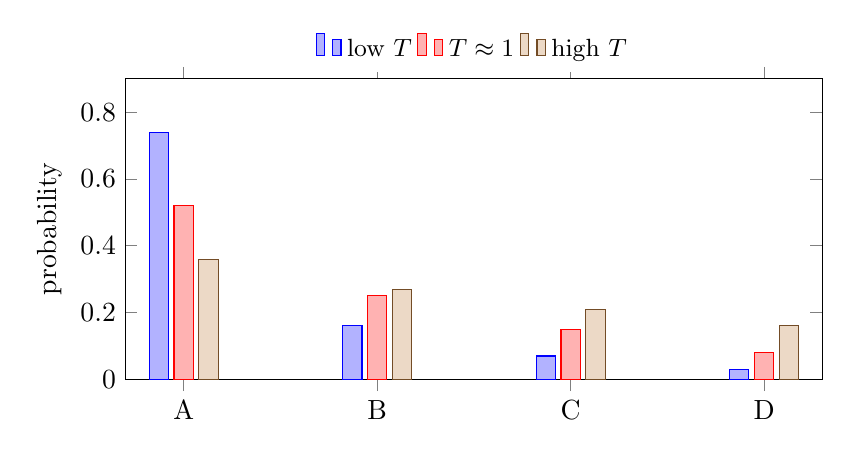
\begin{tikzpicture}
\begin{axis}[
width=.86\linewidth,height=5.4cm,
ybar,bar width=7pt,
ymin=0,ymax=.9,
ylabel={probability},
symbolic x coords={A,B,C,D},xtick=data,
legend style={draw=none,font=\small,at={(.5,1.02)},anchor=south,legend columns=3}
]
\addplot coordinates {(A,.74) (B,.16) (C,.07) (D,.03)};
\addlegendentry{low $T$}
\addplot coordinates {(A,.52) (B,.25) (C,.15) (D,.08)};
\addlegendentry{$T\approx1$}
\addplot coordinates {(A,.36) (B,.27) (C,.21) (D,.16)};
\addlegendentry{high $T$}
\end{axis}
\end{tikzpicture}
\caption{Schematic temperature effect: the same logit ranking becomes sharper at low temperature and flatter at high temperature.}
\label{fig:modern-temperature-distributions}
\end{figure}

\subsubsection{Top-\texorpdfstring{$k$}{k} sampling}
\label{subsec:modern-topk}
Suppose the vocabulary has 100,000 tokens.
Even absurd tokens may receive tiny probabilities.
Top-$k$ says:

\begin{quote}
Keep only the $k$ most probable tokens.
\end{quote}

For $k=3$, keep Jupiter, Saturn and Earth, discard the rest, renormalise and sample.

Its weakness is that a fixed $k$ ignores the shape of the distribution.
Sometimes one answer is obviously correct and keeping 50 tokens is silly.
Other times many continuations are plausible and 50 may be too restrictive.

\subsubsection{Top-\texorpdfstring{$p$}{p} / nucleus sampling}
\label{subsec:modern-topp}
Top-$p$ instead says:

\begin{quote}
Retain the smallest set of tokens whose cumulative probability reaches $p$.
\end{quote}

Suppose:
\[
\begin{array}{rcl}
P(\text{Jupiter})&=&0.55,\\
P(\text{Saturn})&=&0.20\quad(\text{cumulative }0.75),\\
P(\text{Earth})&=&0.10\quad(\text{cumulative }0.85),\\
P(\text{Mars})&=&0.05\quad(\text{cumulative }0.90).
\end{array}
\]

For $p=0.9$, keep those four.
Now consider another distribution where Jupiter already has probability $0.96$.
For the same $p=0.9$, only Jupiter is necessary.

\begin{calloutmemoryhook}
Top-$k$ keeps a fixed number of candidates; top-$p$ keeps a variable number whose probability mass reaches a fixed threshold.
\end{calloutmemoryhook}

So top-$p$ adapts to uncertainty.
That is its core advantage over top-$k$.

\subsection{Beam search}
\label{subsec:modern-beam-search}
Greedy decoding searches one path.
Beam search keeps several promising hypotheses.

\begin{figure}[htbp]
\centering
\begin{tikzpicture}[level distance=11mm,sibling distance=22mm,every node/.style={font=\small}]
\node[flow] {START}
 child {node[yesbox] {A}
   child {node[yesbox] {A1}}
   child {node[yesbox] {A2}}}
 child {node[yesbox] {B}
   child {node[yesbox] {B1}}
   child {node[yesbox] {B2}}}
 child {node[yesbox] {C}
   child {node[yesbox] {C1}}
   child {node[yesbox] {C2}}};
\end{tikzpicture}
\caption{Beam search keeps several high-scoring partial sequences rather than committing to one local choice immediately.}
\label{fig:modern-beam-search}
\end{figure}

At each step, keep the best $N_{\text{beam}}$ partial sequences.
This approximates
\[
\argmax_y p(y\mid x).
\]

Beam search is useful where finding a high-probability complete sequence matters, historically including machine translation.
But for open-ended text, highest-likelihood sequences are not always the most interesting or natural.

\subsection{Decoding map}
\label{subsec:modern-decoding-map}
\begin{figure}[htbp]
\centering
\begin{tikzpicture}[node distance=7mm and 10mm]
\node[flow] (logits) {Model logits};
\node[flow,below=of logits] (temp) {Temperature scaling};
\node[yesbox,below=of temp] (prob) {Probability distribution};
\node[flow,below left=9mm and 17mm of prob] (greedy) {Greedy};
\node[flow,below=9mm of prob] (sampling) {Sampling};
\node[flow,below right=9mm and 17mm of prob] (search) {Search};
\node[yesbox,below left=7mm and 8mm of sampling] (topk) {top-$k$};
\node[yesbox,below right=7mm and 8mm of sampling] (topp) {top-$p$};
\node[yesbox,below=of search] (beam) {beam};
\draw[arr] (logits)--(temp);\draw[arr] (temp)--(prob);
\draw[arr] (prob)--(greedy);\draw[arr] (prob)--(sampling);\draw[arr] (prob)--(search);
\draw[arr] (sampling)--(topk);\draw[arr] (sampling)--(topp);\draw[arr] (search)--(beam);
\end{tikzpicture}
\caption{Decoding choices act after the model has produced logits; they alter the output policy without changing learned weights.}
\label{fig:modern-decoding-map}
\end{figure}

Crucially, decoding can change behaviour without changing the model's weights.
That is why generation settings matter.

\begin{calloutdegreeofexperiment}
For decoding, vary temperature, top-$k$, top-$p$, beam width, stopping rules, repetition penalties and task-specific constraints; compare quality, diversity, determinism and latency rather than treating one setting as universally best.
\end{calloutdegreeofexperiment}




\section{Overview}
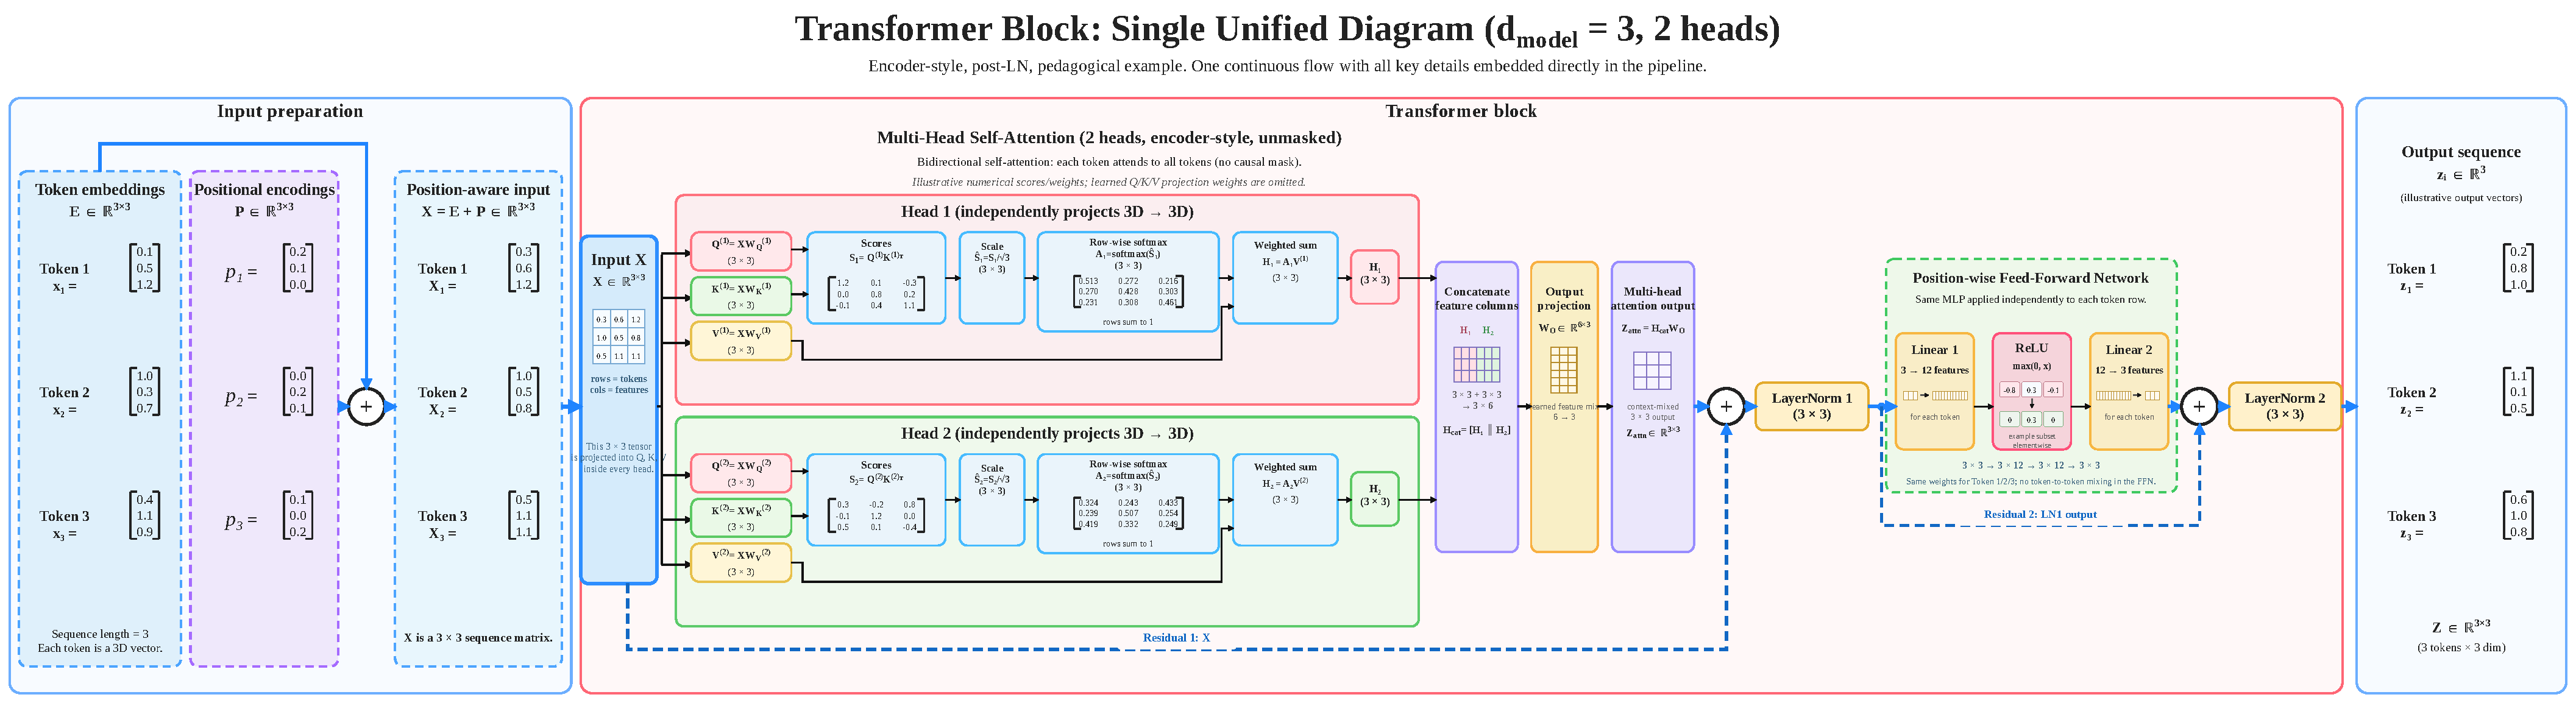
\includegraphics[width=\textwidth]{figures/transformer_format_fixed_v7.pdf}
This is the table worth knowing for research interviews.

\begin{center}
\small
\begin{longtable}{@{}L{.24\linewidth}L{.68\linewidth}@{}}
\toprule
\textbf{Method} & \textbf{Main inductive bias / assumption} \\
\midrule
\endhead
Tokenisation & useful linguistic structure can be represented by chosen discrete units \\
Sinusoidal positions & sequence position has smooth multiscale structure \\
Relative positions & interaction depends importantly on displacement \\
RoPE & query--key similarity should incorporate relative displacement geometrically \\
Causal attention & information flows past $\rightarrow$ future \\
Cross-attention & one representation should selectively retrieve information from another \\
Transformer & arbitrary pairwise content-dependent interactions are useful \\
RNN & history can be compressed into a fixed state \\
S4 & history can be represented through structured dynamical evolution \\
Transformer-XL & earlier hidden states should remain explicitly reusable \\
Griffin & nearby information benefits from attention; long-term information can be recurrently compressed \\
Perceiver & large inputs can be compressed through a latent bottleneck \\
MoE & different inputs benefit from specialised parameter subsets \\
LoRA & useful adaptation lies in a low-dimensional parameter-update space \\
Pretraining & predicting data structure produces reusable representations \\
SFT & desired behaviour can be learned by imitation \\
RLHF & comparative human preference provides a useful behavioural signal \\
FlashAttention & \textbf{no new modelling bias}; implementation optimisation \\
Decoding & \textbf{no training bias}; controls how model probabilities become outputs \\
\bottomrule
\end{longtable}
\end{center}


This is a useful classification when reading papers.

\begin{center}
\small
\caption{Useful classification when reading papers}
\begin{tabularx}{.92\linewidth}{@{}L{.31\linewidth}Y@{}}
\toprule
\textbf{Design layer} & \textbf{Examples} \\
\midrule
Input representation & tokenisation \\
Positional representation & sinusoidal, relative, RoPE \\
Information-flow constraint & causal masking \\
Information source & cross-attention \\
Sequence architecture & Transformer, RNN, S4, Griffin, Transformer-XL \\
Bottleneck architecture & Perceiver \\
Hardware algorithm & FlashAttention \\
Capacity scaling & scaling laws, MoE \\
Training objective/stage & pretraining, SFT, RLHF \\
Parameter adaptation & LoRA \\
Inference policy & temperature, top-$k$, top-$p$, beam search \\
\bottomrule
\end{tabularx}
\end{center}

This taxonomy prevents a lot of category errors.

\begin{calloutexample}
``Is FlashAttention an alternative to causal attention?'' No: causal attention can be executed with FlashAttention.

``Is LoRA an alternative to Transformer?'' No: LoRA can fine-tune a Transformer.

``Is RoPE an alternative to FlashAttention?'' No: one supplies positional structure; the other makes computation efficient.

``Is MoE an alternative to scaling laws?'' No: scaling laws describe empirical behaviour; MoE is one architecture for increasing capacity efficiently.
\end{calloutexample}


Suppose you want to build an LLM capable of reading extremely long scientific papers.
You immediately have many degrees of freedom.

\begin{figure}[htbp]
\centering
\begin{tikzpicture}[node distance=6.5mm]
\node[flow] (data) {DATA\\How much? Quality? Domains?};
\node[flow,below=of data] (tok) {TOKENISER\\32k? 100k? byte fallback?};
\node[flow,below=of tok] (pos) {POSITION\\RoPE? relative? context extension?};
\node[flow,below=of pos] (arch) {ARCHITECTURE\\Transformer? XL? S4-like? Griffin-like?};
\node[flow,below=of arch] (att) {ATTENTION\\global? local? causal? FlashAttention?};
\node[flow,below=of att] (cap) {CAPACITY\\dense? MoE? how many experts?};
\node[flow,below=of cap] (train) {TRAINING\\parameters? tokens? compute balance?};
\node[flow,below=of train] (adapt) {ADAPTATION\\full fine-tune? LoRA? preference training?};
\node[yesbox,below=of adapt] (infer) {INFERENCE\\temperature? top-$p$? context?};
\draw[arr] (data)--(tok);\draw[arr] (tok)--(pos);\draw[arr] (pos)--(arch);\draw[arr] (arch)--(att);\draw[arr] (att)--(cap);\draw[arr] (cap)--(train);\draw[arr] (train)--(adapt);\draw[arr] (adapt)--(infer);
\end{tikzpicture}
\caption{Research optionality is layered: each design decision changes a different part of the system and therefore a different trade-off.}
\label{fig:modern-research-project-optionality}
\end{figure}

This is what \textbf{optionality in system design} actually looks like.
Research generally isn't ``which algorithm is best?''
It is:

\begin{quote}
Which assumptions and resource trade-offs fit this problem?
\end{quote}

\begin{calloutdegreeofexperiment}
For a long-context LLM, vary data/tokeniser, positional method, explicit versus compressed memory, local/global attention structure, kernel implementation, total versus active capacity, parameter/data/compute allocation, adaptation strategy and decoding policy.
Ablate one design layer at a time where possible so architectural and systems effects are not conflated.
\end{calloutdegreeofexperiment}

\section{Final compression}
\label{sec:modern-final-compression}
If you remember only the core distinctions:

\begin{enumerate}
\item \textbf{Tokenisation} chooses the discrete units the model sees.
\item \textbf{Positional methods} tell a permutation-insensitive Transformer about sequence order.
\item \textbf{Sinusoidal} gives structured coordinates; \textbf{relative position} directly represents distance; \textbf{RoPE} turns position into rotations so relative displacement appears naturally in $QK^\top$.
\item \textbf{Causal attention} controls \textit{which tokens may interact}; \textbf{cross-attention} controls \textit{where K/V come from}; \textbf{FlashAttention} controls \textit{how the same computation runs efficiently}.
\item \textbf{RNNs} compress history into state; \textbf{Transformers} keep explicit content-addressable history; \textbf{S4} treats sequence processing as structured state-space dynamics.
\item \textbf{Transformer-XL} adds reusable segment memory; \textbf{Griffin} combines recurrent long-term memory with local attention; \textbf{Perceiver} compresses huge inputs into a small latent workspace.
\item \textbf{Scaling laws} describe predictable empirical relationships between loss, data, parameters and compute.
\textbf{Chinchilla} emphasised that model size and training data must be balanced.
\item \textbf{MoE} separates \textit{total parameter capacity} from \textit{parameters activated for one token}.
\item \textbf{Pretraining} builds general capability; \textbf{fine-tuning} changes behaviour for a narrower distribution; \textbf{LoRA} makes that adaptation low-rank and cheap.
\item \textbf{RLHF} introduces human preference information after pretraining/SFT.
\item \textbf{Decoding} happens after the neural network has produced its probabilities and decides how those probabilities become actual text.
\end{enumerate}

\section{Research evolution: how should sequence information move?}
\label{sec:transformers-evolution}
\begin{center}
\small
\begin{tabularx}{.97\linewidth}{@{}L{.18\linewidth}L{.21\linewidth}YY@{}}
\toprule
\textbf{Step} & \textbf{What changed} & \textbf{Problem targeted} & \textbf{New trade-off} \\
\midrule
RNN & Compress history into recurrent state & Sequence dependence & Sequential bottleneck / long-memory difficulty \\
Attention on RNNs & Directly retrieve useful past states & One-state bottleneck & Added pairwise matching cost \\
Transformer & Make attention the main communication mechanism & Parallel training and direct long-range routes & Dense $N^2$ interaction cost \\
Efficient attention / KV variants & Restrict or share interaction structure & Long-context/serving cost & Extra architectural bias \\
SSM branch & Compress long history into evolving state & Linear-time long sequences & Less explicit all-pairs interaction \\
\bottomrule
\end{tabularx}
\end{center}

\begin{calloutbias}
If useful relationships between sequence elements depend on content, attention can dynamically route information; if most useful interaction is local or compressible into state, unrestricted dense attention may spend unnecessary compute.
\end{calloutbias}

\begin{calloutdegreeofexperiment}
Vary depth, representation width, head count/dimension, attention pattern, positional mechanism, context length, MLP expansion, normalisation/residual placement and key/value sharing.
\end{calloutdegreeofexperiment}

\section{Walkthrough}
Connecting everything: one token through an imaginary modern LLM}
\label{sec:modern-one-token-through-system}
Let's now run a single token through an imaginary modern LLM.
You type:
\begin{quote}
Why is the sky blue?
\end{quote}

\paragraph{Stage A --- tokenisation.}
Raw characters become token pieces and then integer IDs.
The tokenizer determines the atomic units.

\paragraph{Stage B --- embeddings.}
Each ID becomes a vector
\[
x_i\in\mathbb R^{N_{\text{representation dims}}}.
\]

\paragraph{Stage C --- positional information.}
Suppose the model uses RoPE.
Queries and keys are rotated according to their positions.

\paragraph{Stage D --- causal attention.}
For every token, calculate scaled query--key compatibility, then apply the causal mask so future positions are forbidden.

\paragraph{Stage E --- efficient execution.}
The implementation may use FlashAttention: the same mathematical attention is tiled to reduce memory traffic.

\paragraph{Stage F --- next-token probabilities.}
The final hidden state is projected to vocabulary logits, then softmax produces $P(\text{next token})$.

\paragraph{Stage G --- decoding.}
Perhaps temperature and top-$p$ are applied, a token is sampled, appended, and the process repeats.

\begin{figure}[htbp]
\centering
\resizebox{.97\linewidth}{!}{%
\begin{tikzpicture}[node distance=6mm and 7mm]
\node[flow] (prompt) {Prompt};
\node[flow,right=of prompt] (tok) {Tokenise};
\node[flow,right=of tok] (emb) {Embedding};
\node[flow,right=of emb] (rope) {RoPE};
\node[flow,right=of rope] (att) {Causal attention\\via FlashAttention};
\node[flow,right=of att] (logit) {Vocabulary\\logits};
\node[flow,right=of logit] (dec) {Temperature\\+ top-$p$};
\node[yesbox,right=of dec] (next) {Next token};
\draw[arr] (prompt)--(tok);\draw[arr] (tok)--(emb);\draw[arr] (emb)--(rope);\draw[arr] (rope)--(att);\draw[arr] (att)--(logit);\draw[arr] (logit)--(dec);\draw[arr] (dec)--(next);
\draw[arr,rounded corners] (next.south)--++(0,-.7)--([yshift=-.7cm]prompt.south)--(prompt.south);
\end{tikzpicture}}
\caption{One autoregressive generation loop with the major mechanisms from this chapter attached to their actual place in the data flow.}
\label{fig:modern-one-token-loop}
\end{figure}


























